\documentclass[a4paper,11pt]{article}
\usepackage{parskip}
\usepackage{a4wide}
\usepackage[named]{algo}
\usepackage{graphicx}
\usepackage{subfig}

\title{Geometric Algorithms - 2IL55\\Spanner project}
\author{Matias Piispanen\\Marieke Zantema}
\date{Spring 2011}

\begin{document}
%{\centering{
%{\LARGE{Geometric Algorithms - 2IL55\\Spanner project}}
%\newline
%{\large{\\Matias Piispanen\\Marieke Zantema\\}}
%}}
\begin{titlepage}
\maketitle
\end{titlepage}

\section{Introduction}
Networks can be found in all sorts of everyday problems. Whenever it comes to connecting `things' to each other -- cities connected by railroads, computers connected by cables, buildings connected by the sewer -- the problem is a network problem. In almost all cases it is not feasible to connect all nodes to all other nodes, so it will be necessary to construct a better network. It is often desired to have a small size (number of railroads, cables or pipes), a small weight (amount of railroad) and a small dilation (the distance via the network should not be more than the real distance multiplied by a constant $t$).
We implement three different algorithms to make a network with a given maximum dilation $t$, or $t$-spanner for short. One algorithm is based on an s-Well Separated Pair Decomposition (s-WSPD for short), another is a greedy algorithm and the third algorithm is a theta spanner. To test our algorithms, we generate random points and look at the properties of the spanners created by the various algorithms.
\\
\\During our experiments we found that the actual running time of the theta spanner to construct spanners is shortest out of the tested algorithms and in most cases it also produces spanners with the best quality measurements. The s-WSPD based spanner also works relatively fast, but in general cases it produces spanners with a very large size and it works better with datasets that are known to be more suitable for this sort of an algorithm. The greedy spanner algorithm was observed to be suitable for very small datasets only, because its running time is so large.

\section{The algorithms}

\subsection{WSPD-based}

A WSPD-based spanner algorithm first constructs an s-Well Separated Pair Decomposition and then simply connects representatives of each found pair sets with an edge.

The algorithms presented in the lecture slides will be used to implement the WSPD-based spanner algorithm. The s-Well Separated Pair Decomposition algorithm is based on constructing a quadtree and identifying which nodes make a well separated pair. Two sets $A$ and $B$ form an s-Well Separated Pair if $A$ and $B$ are s-Well Separated: there exist such balls $D_A$ and $D_B$ that enclose the points in $A$ and $B$, respectively, so that $d(D_A, D_B) \geq s \cdot max(radius(D_A), radius(D_B))$ holds. The following algorithm for finding the s-Well Separated Pairs was presented on the lectures:
\pagebreak
\begin{algorithm}{wsPairs}{
  \qprocedure{wsPairs}
  \qinput{$u$, $v$, Quadtree $T$, $s$}
  \qoutput{s-Well Separated Pair Decomposition $W$}
}
\qif $repu(u)$ or $rep(v)$ is $empty$ \\
  \qreturn $\emptyset$ \\
\qelse \qfi \qif $u$ and $v$ are s-Well Separated \\
  \qreturn ($u$, $v$)  \qfi \\
\qif $level(u) < level(v)$ \\
  swap $u$ and $v$ \qfi \\
Let $u_1, u_2, ..., u_m$ denote the children of $u$ in $T$ \\
\qreturn $Sum_i$ wsPairs($u_i$, $v_i$, T, s)
\end{algorithm}

The algorithm will be generated using a regular uncompressed quadtree in $O(d+1)n$ running time where $d$ is the depth of the quadtree. The algorithm could be made more efficient by using compressed quadtrees which makes the running time of the s-WSPD construction $O(n \log n + s^d n)$. After the s-WSPD has been constructed, the spanner can be generated by simply connecting one representative of each pair set to another with the following algorithm. The representatives were chosen randomly.

\begin{algorithm}{WSPD-Spanner}{
  \qprocedure{WSPD-Spanner}
  \qinput{Point set $V$, $t  > 1$}
  \qoutput{t-Spanner $G(V,E)$}}
  $s \qlet 4\cdot (t+1)(t-1)$ \\
  $W \qlet wsPairs(root_T, root_T, T, s)$ \\
  $E \qlet \emptyset$ \\
  \qfor ($A_i, B_i$ in $W$ \\
  Select arbitrary node $u$ in $A_i$ and $v$ in $B_i$ \\
  Add edge ($u, v$) to $E$ \qfi \\
  \qreturn $G(V, E)$
\end{algorithm}

An implementation of the WSPD based spanner algorithm with a regular uncompressed quadtree has running-time of $O((d-1) n) + s^d n)$.

\subsection{Greedy spanner}

The greedy algorithm is the simplest, and also the slowest, algorithm for constructing a geometric spanner. It is still a good comparison for the more complex algorithms for seeing how much better quality spanners they can construct compared to the greedy algorithm.

The greedy algorithm starts by listing all point pairs based on their distance. The initial spanner graph has no edges. The algorithm then checks for each point pair whether the dilation for that pair is greater than $t$ and adds an edge between them if it is.

There are $n^2$ pairs that have to be compared. Finding a shortest path with Dijkstra's algorithm takes $O(|E| + n \log n)$ time, where $|E|$ is the number of edges, so the total running time of the algorithm is $O(n^2(|E| + n \log n))$.

\subsection{Theta spanner}
To construct a theta spanner for the given set of points and the given required dilation, first the required number of cones is calculated. For this, we use the formula $t \leq 1/(1-2\sin(\theta/2))$, which can be rewritten to $k \geq \pi/(\arcsin(1/2-1/2t))$ where $\theta=2\pi/k$. This is used to calculate the minimum number of cones needed. Please refer to the appendix for details about this formula.
\\We have an algorithm that calculates the leftmost point in a cone (details about this algorithm will be discussed later), so for each cone, we need to rotate all points about the origin until the bisector of the cone is a ray in positive $x$-direction. The coordinates are no integers anymore, so each \verb'Point' is converted to a \verb'Punt': a pair of doubles representing the $x$- and $y$-coordinates. To keep track of which \verb'Point' is represented by which \verb'Punt', we need the type \verb'IndexedPunt'. This is a pair consisting of a \verb'Punt' and an integer \verb'index', such that the \verb'Point' at \verb'points[index]' corresponds to the \verb'Punt'. All \verb'Point's are stored as \verb'IndexedPunt'en in the array \verb'Punten'.
\\After the rotation, one of the cone's rays lies above the bisector; this ray is called $r_1$, and the other ray ($r_2$) lies below the bisector. If the rays of the cones are `nice' lines, like horizontal or vertical lines, or lines with a `nice' slope like 1 or 3/2, it can happen that there are points exactly \textit{on} a ray. Recall that the coordinates of the points originally were integers, but are converted to doubles because of the rotation. Due to rounding errors it may lead to incorrect theta spanners if there are points on rays, so it is important that the rays are `non-nice' lines. This is done by rotating the points an extra 0.1 radians. In other words, the cones are chosen such that the bisector of the first cone lies 0.1 radians below a horizontal line (with respect to the original integer points).
\begin{figure}[h]
\centering
\includegraphics[width=0.8\textwidth]{Cones}
\caption*{Rotating the cones.}
\end{figure}
\\For each of the $k$ orientations, a sweep-line algorithm is used to find for each point the leftmost point in the cone. This algorithm is illustrated in the picture below. The sweep line is parallel to $r_1$ and sweeps in positive $x$-direction. So the event queue of this algorithm is a vector that stores all points, sorted by `distance' from $r_1$ where the `distance' is negative if the point lies above $r_1$.
\\The status is a non-trivial data structure, illustrated in the picture below. It starts as a binary tree but its leaves and internal nodes are `cut away' when the sweep line algorithm is being executed. The points are stored in the leaves of this tree and they are sorted by `distance' from $r_2$. Each node contains two points: the leftmost (smallest $x$-coordinate) point of the subtree plus the point that is leftmost in the subtree (but does not necessarily have the smallest $x$-coordinate). For example, the root node contains $(1, 7)$, which means that point 1 is leftmost and point 7 is leftmost in the tree. Note that the real tree stores the coordinates of the points: the leftmost point is stored as an \verb'IndexedPunt' and the point that is leftmost in the tree is stored as a \verb'Punt'.
\\Only one operation is needed on this datastructure: $\textsc{Update}(p)$. Note that this operation is integrated in the code, so there is no actual function \textsc{Update}, but it is easier to discuss a function than `the part of the code that\dots'. The `function' \textsc{Update} involves searching for the point $p$ in the tree by walking from the root to the leaf where $p$ is stored, deleting $p$, and going back to the root. Since it is not necessary to add points, deleting a point involves only deleting and not re-building the tree such that it remains a binary tree. The depth of the tree does not increase, so \textsc{Update} always runs in $O(\log n)$ time. When walking from $p$ to the root, the tree is updated (the leftmost point stored in an internal node may have to be changed, or an internal node may have to be deleted) and the leftmost point in the cone is searched for and stored in the \verb'IndexedPunt LeftMostSoFar'. Updating and searching the leftmost point is a huge case distinction: if a node doesn't have children, the node should be removed; if a node has only one child, the child is copied to the node and if the only child is the right child and the algorithm `came from the left', i.e. the left child was handled (removed) in the previous iteration, then \verb'LeftMostSoFar' becomes the first point in the right child. If a node has two children, then the first point of that node becomes the leftmost point of the first points in both children and the second point becomes the second point in the left child. Further, if the algorithm `came from the left', then \verb'LeftMostSoFar' should be compared to the first point of the right child; if the first point in the right child lies further left than \verb'LeftMostSoFar', then \verb'LeftMostSoFar' should become the first point in the right child.
After the root is handled, the tree is updated and the leftmost point to the right of $p$ is stored in \verb'LeftMostSoFar'.
\\An event occurs when the sweep line reaches a point $p$. Then $\textsc{Update}(p)$ is called, and the edge from $p$ to the leftmost point is added to the set of edges, if the cone ins't empty and the edge wasn't there already. The length of the edge is added at the appropriate places in the adjacency matrix.
\begin{figure}[h]
\centering
\includegraphics[width=0.9\textwidth]{ThetaExplain}
\caption*{The sweep-line algorithm (left) and the corresponding status and event queue.}
\end{figure}
%\\Each node in the tree contains two points: the leftmost point and the point that is leftmost in the subtree. For example, the root node contains $(1, 7)$, which means that point 1 is leftmost and point 7 is leftmost in the tree. Note that in the real tree, the leftmost point is stored as an \verb'IndexedPunt' and the point that is leftmost in the tree is stored as a \verb'Punt'. When the sweep line reaches point 1, \textsc{Update} searches for point 1 (guided by the second point in each node). It then deletes the leaf containing point 1 and updates the parent nodes (the updates are below the updated nodes in the picture), and it searches for the leftmost point that lies in the cone (guided by the first point in each node).
\\The theoretical running time of the whole algorithm is $O(kn \log n + n^2)$: for each of the $k$ cones, it sweeps over the points and handles each of the $n$ events (points) in $O(\log n)$ time. The algorithm also generates an ($n \times n$) adjacency matrix.

\section{Experimental setup}
We have written code that generates a text file in the following format. The first line contains one integer, namely the number of points. The second line contains two integers, $a$ and $b$, that indicate the maximum dilation $t=a/b$. The remaining lines contain the points, that is, each line contains two positive integers: the $x$- and $y$-coordinate of the point. Note that this is the same format as the format for the data challenge.
The points for the text file are generated randomly, but the code asserts that no two points are the same. When calling the function GenerateData, one must specify the number of points, the maximum value of $t$ and the maximum value of the $x$- and $y$-coordinates.

We are testing the spanners with respect to their size, weight, maximum degree and the dilation. The actual running times of the algorithms will also be measured by running the algorithms multiple times and calculating the total and average running times.

The GLUT API is used to get inputs from keyboard and visualizing the spanners by using the OpenGL library.

For theta spanners, we have seen that the maximum dilation in the theta spanner can be much lower than the required dilation. We therefore wonder whether we can reduce the number of edges by calculating the theta spanner with a smaller number of cones, and adding edges if the maximal dilation exceeds the required dilation. A disadvantage of such a greedy theta spanner or \textit{gheta spanner} is that it is (theoretically) much slower than a theta spanner. Calculating the maximal dilation has a theoretical running time of $O(n^3)$, whereas a theta spanner theoretically is generated in $O(kn\log n + n^2)$ time.
\\We will first investigate by how much we can reduce the number of cones: for a number of theta spanners we will calculate the minimum number of cones needed to achieve the required dilation $(N)$ and we will compare this to the upper bound as given by the formula $(F)$. The ratio $F/N$ tells us by how much we can reduce the number of cones.
\\To compute the number of cones that is needed, we calculate the maximum dilation for several numbers of cones, starting at the number of cones given by the formula, and halving the number of cones as long as the maximal dilation is less than the required maximum dilation. When, for some number of cones, the maximal dilation is larger than the required dilation, the algorithm binary-searches for the minimum number of cones needed. We assume that each combination of a point set and a required dilation has a minimum number of cones $k_c$, so theta spanners with less than $k_c$ cones have a maximal dilation that is larger than the required dilation and theta spanners with $k_c$ or more cones have dilations that are smaller than the required dilation.

\section{Results and discussion}
\subsection{Data challenge}
The results of the data challenge can be found in the tables below.
\pagebreak
\\
\\ClusterGridPlusTwo
\\\begin{tabular} {| l || l | l | l |}
\hline
Spanner & Greedy & WSPD & Theta \\ \hline \hline
Size & 5678 & 3847 & 512 \\ \hline
Weight & $5.32\cdot 10^5$ & $3.14\cdot 10^5$ & $3.00\cdot 10^4$ \\ \hline
Max. degree & 101 & 90 & 16 \\ \hline
Max. dilation & 1.57 & 1.49 & 1.70 \\ \hline
\end{tabular}
\\
\\Cities in the Netherlands
\\\begin{tabular} {| l || l | l | l |}
\hline
Spanner & Greedy & WSPD & Theta \\ \hline \hline
Size & 907 & 5070 & 538 \\ \hline
Weight & $1.44\cdot 10^6$ & $3.00\cdot 10^7$ & $9.59\cdot 10^5$ \\ \hline
Max. degree & 27 & 119 & 13 \\ \hline
Max. dilation & 1.88 & 1.68 & 1.42 \\ \hline
\end{tabular}
\\
\\Train stations in the Netherlands
\\\begin{tabular} {| l || l | l | l |}
\hline
Spanner & WSPD & Theta \\ \hline \hline
Size & 17512 & 3524 \\ \hline
Weight & $3.82\cdot 10^8$ & $2.92\cdot 10^7$ \\ \hline
Max. degree & 216 & 58 \\ \hline
Max. dilation & 1.96 & 1.24 \\ \hline
\end{tabular}
\\
\\The file with the train stations contained some duplicates, which were removed. Our implementation of theta spanner can't deal with duplicates. We have no data for the greedy spanner, because it still wasn't finished after 3,5 hours.

\subsubsection{Spanner Quality Measures}
The implemented spanners ended up generating quite different kinds of spanners. The following table shows the quality measures for a dataset of 100 points with a required dilation of 1.5. The tables in Section 4.1, which represent more real-life like and special cases, were also used in the analysis and discussion in the following subsections.
\\
\\Spanner Measures
\\\begin{tabular} {| l || l | l | l |}
\hline
Spanner & Greedy & WSPD & Theta \\ \hline \hline
Size & 386 & 3818 & 935 \\ \hline
Weight & 443240 & $1.75\cdot 10^7$ & $1.97\cdot 10^6$ \\ \hline
Max. degree & 14 & 95 & 32 \\ \hline
Max. dilation & 1.44 & 1.24 & 1.10 \\ \hline
\end{tabular}
\paragraph{Greedy spanner}
The quality of the spanners constructed by the greedy algorithm is a mixed bag. With a randomized dataset it constructs considerably smaller spanners than the other two algorithms with much lower size, weight and maximum degree values. In a more realistic task like connecting building a spanner of all the cities in the Netherlands the resulting spanner is $69\%$ larger than the theta spanner, although still considerably smaller than the WSPD based spanner. The ClusterGridPlusTwo dataset shows that there are cases where the greedy spanner algorithm behaves poorly. In this case it is the grid structure that the greedy algorithm handles poorly. The size of the spanner generated on this dataset is over 10 times the size of the theta spanner and almost twice the size of the WSPD spanner.
\\
\\The strengths of the greedy algorithm are that it is very simple to implement and you can expect fairly good quality spanners. If the dataset is known to be more or less random, you can even expect superior spanners compared to the other observed spanner algorithms in terms of size, weight and maximum degree. However as the running time of the algorithm is $O(n^2(|E| + n \log n))$, the algorithm is quite useless with large datasets.
\paragraph{Theta spanner}
Apart from the randomized dataset, the theta spanner produces spanners with clearly the best quality measurements. The spanners are very compact and because the algorithm connects points closest to the itself in each cone, the maximum degree of the spanners also stays very low.
\\
\\In conclusion the theta spanner seems to construct spanner with very good quality values with a very fast running time.
\paragraph{WSPD-based spanner}
The spanners generated with the s-Well Separated Pair Decomposition based approach turned out to be very large. With a randomized dataset the size of the WSPD based spanner turned out to be almost 10 times the size of the greedy algorithm with the weight and maximum degree also considerable higher than with the other algorithms. With the Cities in the Netherlands dataset the size of the resulting spanner is equally high. This was unexpected behaviour compared to the expectations we had at the beginning of the project.
\\
\\The unexpectedly large sizes of the WSPD based spanners can be explained by observing the formula that gives the multiplier for the distance between the pairs which is $s = 4\cdot(t+1)/(t-1)$. For example if the maximum allowed dilation $t$ is 1.5, the formula gives $s=20$. This means that the pair for a set of points $A$ which can be enclosed inside a ball $D_A$ has to to lie at least $20\cdot radius(D_A)$ away from both of the points.
\\
\\While the sizes of the WSPD based spanners are still much higher than the sizes of the theta spanners with the remaining two datasets, they do give hope that there might indeed be datasets that give reasonably good results with the WSPD based algorithm. The algorithm gives better spanners if the points in the datasets are clustered and the clusters are far enough from each other, so they form well separated pairs with each other. For example, if the dataset of the train stations had been from a country where major cities have lots of stations for short-distance trains while the distances between cities are larger, then you could have expected the WSPD based algorithm to produce a much smaller spanner, as the train stations would have been clustered around the cities.
\\
\\In conclusion, the WSPD algorithm is a reasonably fast algorithm but for most datasets it constructs unreasonably large spanners. It should only be used if there's prior knowledge that the dataset is clustered and the distances between the clusters are reasonably large compared to their diameter.

\subsection{Running times}
\subsubsection{Greedy spanner}
The theoretical running time of the greedy spanner algorithm is $O(n^2(|E| + n \log n))$. The running time of the algorithm was tested with randomized point sets of sizes from 0 to 100. The running time has polynomial growth and the rate of growth is quite steep. It was already observed that a spanner on a dataset of 388 points takes many hours to construct even on modern computers, so one can assume that the observed growth continues. This is expected as the theoretical running time of the algorithm is quite bad.
\\\begin{figure}[h]
\centering
\includegraphics[width=.45\textwidth]{greedy}
\end{figure}
\subsubsection{WSPD based spanner}
The theoretical running time of WSPD based spanner is $O((d-1) n) + s^d n)$. The WSPD based spanner was tested by constructing the spanner with varying number of points. The noise in the resulting graph is due to the fact that the spanner was created only once with a random point set of each size between 0 and 300. This is however not important as the results are still very clear. As the amount of points grows, the minimum distance between any pair of points has a higher probability of being smaller, which makes the depth of the resulting quadtree larger. For this reason the running time of the algorithm does not depend linearly on the amount of points.
\\\begin{figure}[h]
\centering
\includegraphics[width=.45\textwidth]{wspd}
\end{figure}
\pagebreak

\subsubsection{Theta spanner}
The theoretical running time of theta spanner is $O(kn\log n + n^2)$. Two types of test runs were done: runs where the number of points was fixed and the number of cones was varied, and runs where the number of cones was fixed and the number of points was varied. The results can be found in the graphs below; the blue line represents the best linear fit when the number of points is fixed and the best quadratic fit when the number of cones is fixed.
\\\begin{figure}[h]
\centering
\subfloat{\includegraphics[width=.45\textwidth]{ThetaTimeCones}}
%\hspace{15mm}
\subfloat{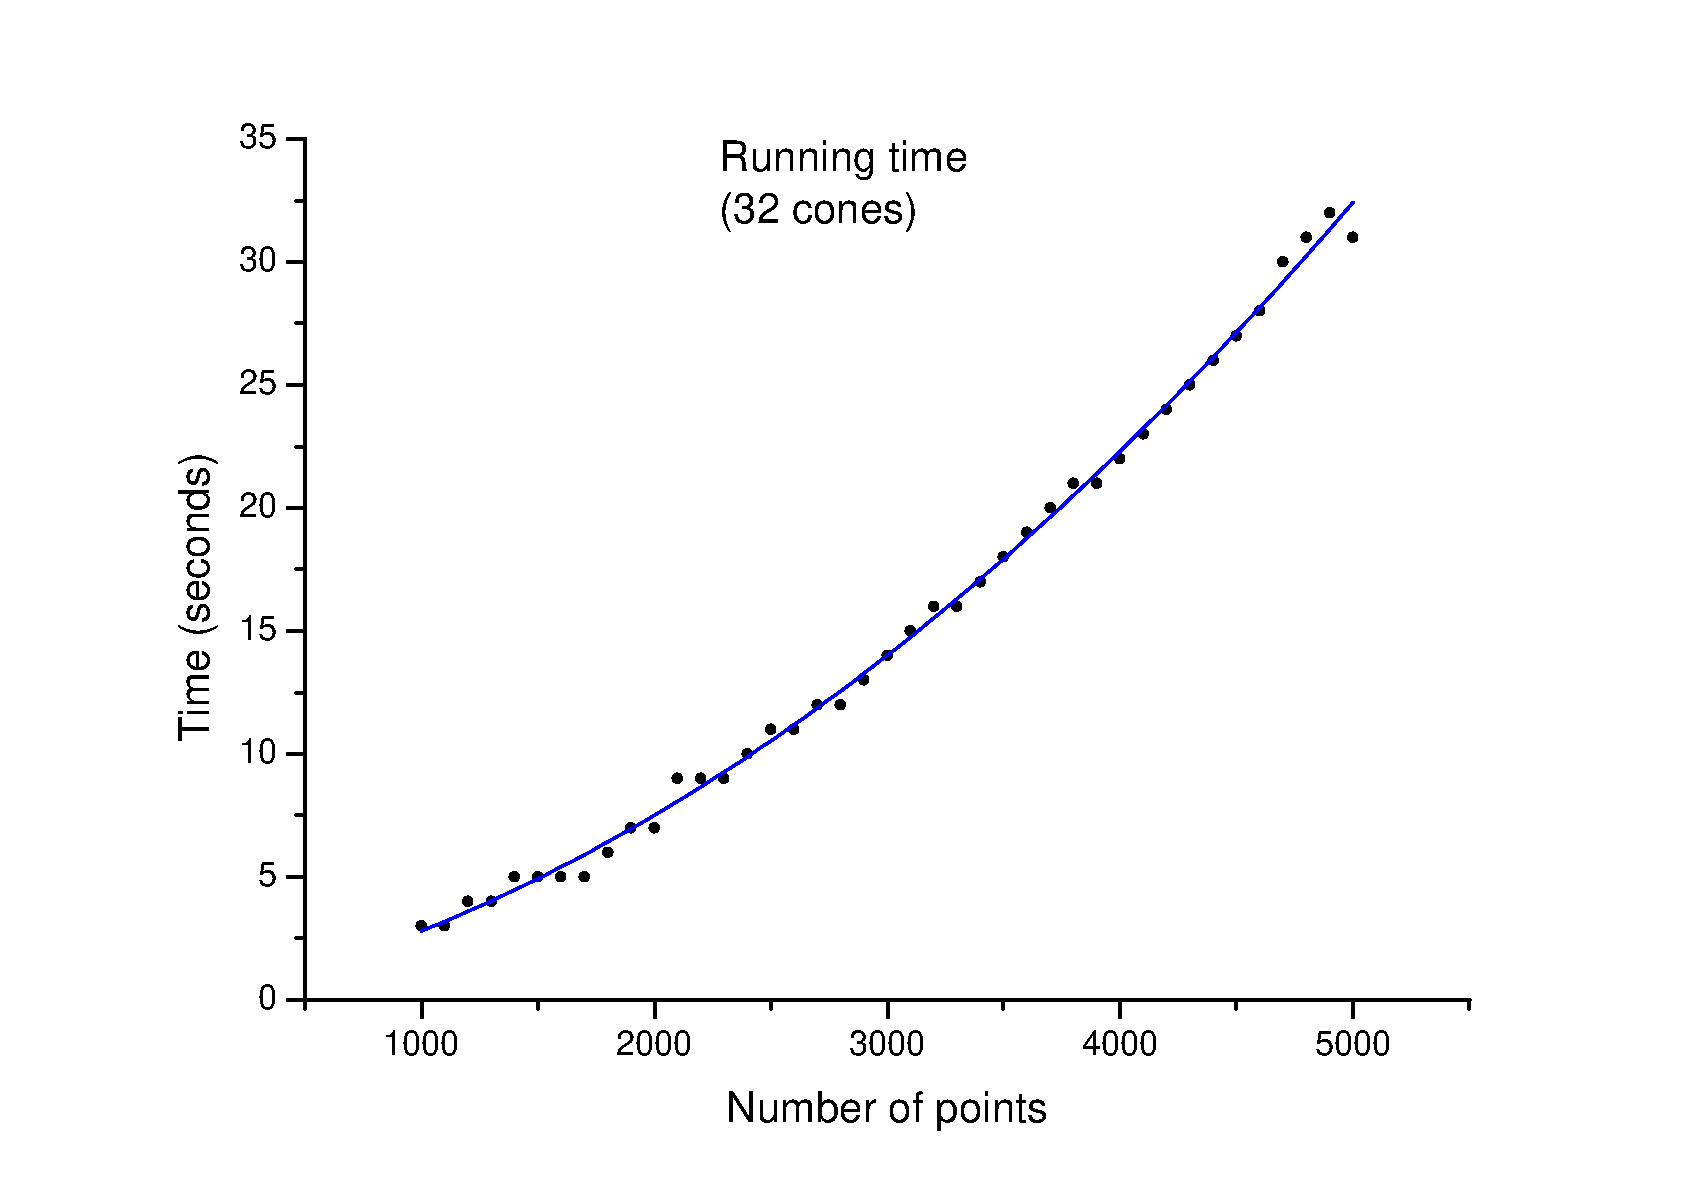
\includegraphics[width=.45\textwidth]{ThetaTimePoints}}
\end{figure}
\\The horizontal lines are caused by the fact that my code can only measure an integer number of seconds. Apart from that, the fit lines nicely go through the points, so the running time indeed depends linearly on the number of cones and quadratically on the number of points.

\subsubsection{Comparison}
The comparison of the actual running times of the three implemented algorithms were tested by running the algorithms with  random point sets multiple times and and timing the total time it took to construct the spanners. The point sets in the tests contained 100 points, because with larger datasets the greedy spanner gets so slow that it takes too much time to run the tests. The maximum dilation of 1.5 was chosen quite arbitrarily. The tests were run 100 times and the total and average running times were calculated. The results can be found in the table below:
\\
\\Actual Running Times
\\\begin{tabular} {| l || l | l | l |}
\hline
Spanner & Theta & Greedy & WSPD \\ \hline
Average & 0.006904s & 7.01425s & 0.20872s \\ \hline
Total & 0.690399s & 701.425s & 20.8715s \\ \hline
\end{tabular}
\\
\\The differences in the running times are quite notable. The greedy spanner is considerably slower than the other two algorithms. Since the total theoretical running time of the greedy algorithm is $O(n^2(|E| + n \log n))$, this was quite expected. The running time difference between the theta and WSPD spanners in favour of the theta spanner probably follows from the fact that the well-separated pairs were found by constructing an uncompressed quadtree. Modifying the algorithm to use compressed quadtrees would probably close the gap between the two algorithms.
\\
The conclusions one can make from these results are that the greedy algorithm should only be used if the datasets are very small. If running time is critical, then constructing the spanners with a theta spanner algorithm might be advisable.

\subsection{Gheta spanners}
We made theta spanners for 55 random point sets. For each theta spanner, we calculated how many cones were needed according to the formula $(F)$ and how many were really needed $(N)$. The point sets contained between 4 and 997 points, and the required dilations varied from 1.017 to 2. Each point in the graph below represents a theta spanner.
\\\begin{figure}[h!]
\centering
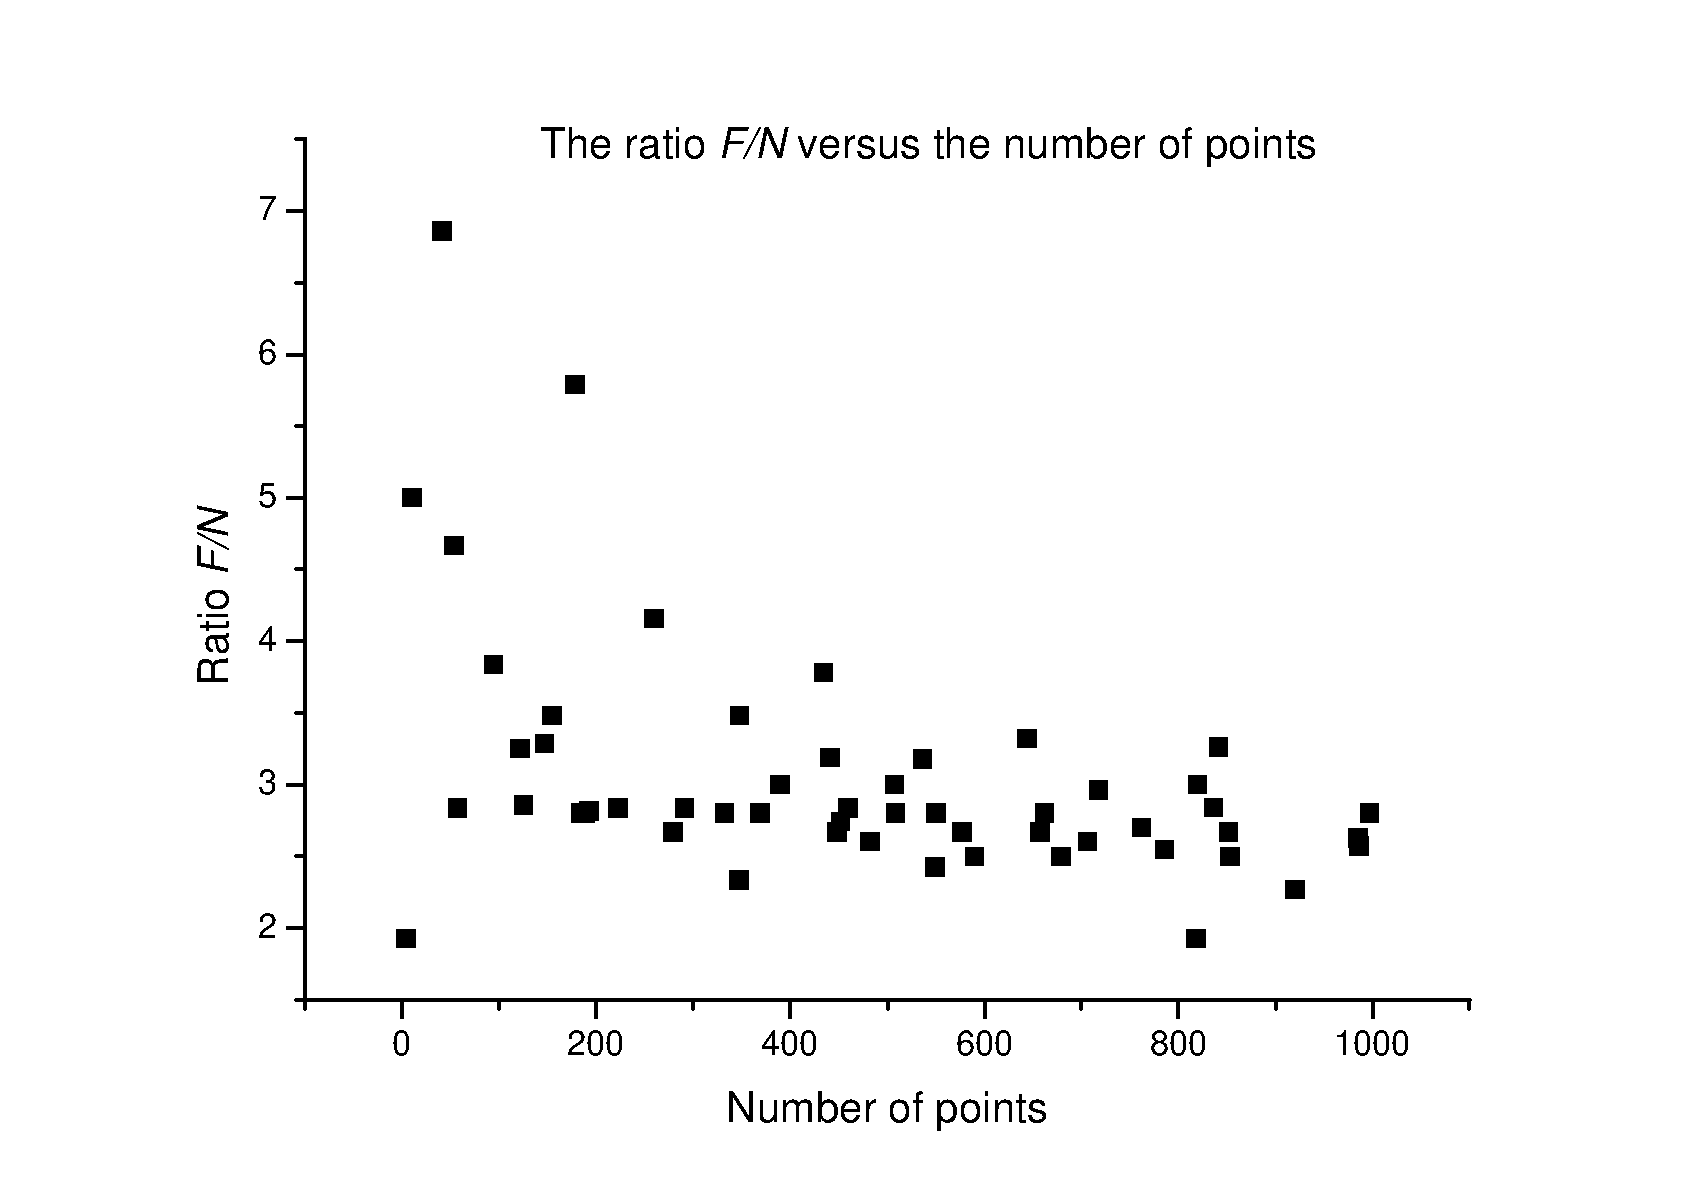
\includegraphics[width=0.8\textwidth]{Needed}
\end{figure}
\\For random sets of points, the number of cones needed to achieve the required dilation is nearly always a factor 2.5 lower than the maximum number of cones given by the formula. This seems to suggest the heuristic to use a \textit{greedy factor} of 2.5, or $F/2.5$ cones, then calculate the maximal dilation and add a \textit{shortcut edge} between two points if the dilation exceeds the maximal dilation. However, a greedy factor of 2.5 would mean that, in most cases, no shortcut edges have to be added at all. A larger greedy factor increases the number of shortcut edges that have to be added, and it greatly reduces the number of `normal' edges. We use a greedy factor of 4.
\\We generated 100 new random point sets, and for each point set we computed both the theta spanner and the gheta spanner. The sizes of the point sets varied from 10 to 976 points and the required dilations were between 1.013 and 1.78. For each spanner we measured the running time, maximal dilation, size, weight and maximal degree, and for each metric we calculated the ratio between the value for the theta- and gheta spanner. The results can be found in the graph below.
\\\begin{figure}[h!]
\centering
\includegraphics[width=0.9\textwidth]{ThetaVsGheta}
\end{figure}
\\Gheta spanners with a greedy factor of 4 reduce the number of edges by a factor 2,8 on average, which is a very nice result. The weight and maximal degree are on average reduced by a factor of 4.9 and 2.7, respectively. The maximal dilation increases a bit when using a gheta spanner, namely a factor on 1.2 on average, but by construction the maximal dilation remains smaller than the required maximal dilation. The only disadvantage of gheta spanner is that it's much slower than a theta spanner: gheta spanner has a running time of $O(n^3)$.
%\\\begin{figure}
%\centering
%\includegraphics[width=0.9\textwidth]{ThetaVsGhetaTime}
%\end{figure}

\clearpage
\section*{Appendix A. The number of cones in a theta spanner}
A derivation of $t \leq 1/(1-2\sin\theta/2)$ can be found in the article by J. Ruppert and R. Seidel, \textit{Approximating the $d$-dimensional complete Euclidean graph}, in \textit{Proceedings of the Third Canadian Conference on Computational Geometry}, pages 207-209, 1991. I give an other derivation, which is in my opinion more intuitive.
\\First consider the triangle $pqr$ in the picture below. Let $p$ and $q$ be arbitrary points, and let $r$ be the leftmost point that lies in the same cone as $q$. We first want to know the worst-case dilation when going from $p$ to $q$ via $r$. Let $\alpha$ and $\beta$ be the angles as defined in the picture; both angles are positive in the picture, but can get negative (if $r$ lies below the bisector of the cone then $\alpha$ is negative, $\beta$ can become negative in a similar way). Let $s=|pr'|/|pq'|$, so we have the following constraints:
\\$0 \leq s \leq 1$ and $-\theta/2 \leq \alpha, \beta \leq \theta/2$, where $0 < \theta \leq \pi/3$.
\\\begin{figure}[h]
\centering
\includegraphics[width=0.5\textwidth]{ConesInTheta}
\end{figure}
\\If 1 unit length is defined as $|pq|$, then:
\\$|pq'|=|\cos \beta|$
\\$|pr'|=|s \cos \beta|$
\\$|pr|=|{\frac {s \cos \beta} {\cos \alpha}}|$
\\$|rr'|=|\sin \alpha {\frac {s \cos \beta} {\cos \alpha}}|$
\\$|qq'|=|\sin \beta|$
\\$|r'q'|=(1-s)|\cos \beta|$
\\$|rq|=\sqrt{\cos^2\beta (1-s)^2 + ({\frac {s \cos \beta \sin \alpha} {\cos \alpha}} + \sin \beta)^2}$
\\Yielding that the dilation $t=|pr| + |rq|=|{\frac {s \cos \beta} {\cos \alpha}}|+\sqrt{\cos^2\beta (1-s)^2 + ({\frac {s \cos \beta \sin \alpha} {\cos \alpha}} + \sin \beta)^2}$. In the domain of $-\theta/2 \leq \alpha, \beta \leq \theta/2$ and $0 \leq s \leq 1$, this function is at most $1+2\sin \theta/2$ and this maximum occurs at $(s, \alpha, \beta)=(1, \theta/2, \theta/2)$ or $(1, -\theta/2, -\theta/2)$. This means that the dilation is maximal when $r$ and $q$ lie on the edges of the cone and equally far from $p$. To prove the maximal dilation in a theta spanner, we assume that the points are arranged such that the dilation is indeed maximal.
\\The \textit{cone path} from $p$ to $q$ (with $p \neq q$) is recursively defined as follows: if there is an edge between $p$ and $q$, this edge is the cone path. If there is no edge from $p$ to $q$, then there is a (unique) point $r$ that lies in the same cone as $q$ and closest to $p$. The cone path is then the edge $pr$ plus the cone path from $r$ to $q$. Note that the cone path is not necessarily the shortest path. Let $l$ be the number of edges in the cone path from $p$ to $q$ and let $|\widetilde{pq}|$ denote the length of the cone path from $p$ to $q$. Then I will prove by induction that for two arbitrary points $p$ and $q$ in a theta spanner:
\[t = {\frac {|\widetilde{pq}|} {|pq|}} \leq \sum_{i=0}^{l-1} (2\sin \theta/2)^i\]
\\Base case, $l=1$. The points $p$ and $q$ are connected by an edge and the dilation trivially is $1=\sum_{i=0}^{l-1} (2 \sin \theta/2)^i$.
\\Induction step, $l > 1$. Let $r$ be the point that lies in the same cone as $q$ and closest to $p$, so the cone path from $p$ to $q$ will go via $r$.
\\\begin{figure}[h]
\centering
\includegraphics[width=0.5\textwidth]{ConesInThetaInductionStep}
\end{figure}
\\For the cone path from $p$ to $q$, we know:
\[|\widetilde{pq}|=|pr| + |\widetilde{rq}|\]
Applying the induction hypothesis gives
\[\leq |pr| + |rq| \sum_{i=0}^{l-2} (2\sin \theta/2)^i\]
\[=|pr| + |rq| + |rq|\sum_{i=1}^{l-2} (2\sin \theta/2)^i\]
Apply the worst-dilation assumption; replace $|pr|+|rq|$ by $|pq|\cdot(1+2\sin\theta/2)$ and replace $|rq|$ by $|pq| \cdot 2\sin\theta/2$
\[\leq |pq|\cdot(1+2\sin\theta/2) + |pq| \cdot 2\sin\theta/2 \sum_{i=1}^{l-2} (2\sin \theta/2)^i\]
\[= |pq|\cdot(1+2\sin\theta/2) + |pq|\sum_{i=2}^{l-1} (2\sin \theta/2)^i\]
\[=|pq|\sum_{i=0}^{l-1} (2\sin \theta/2)^i\]
which proves that $|\widetilde{pq}|/|pq| \leq \sum_{i=0}^{l-1} (2\sin \theta/2)^i$. If the number of edges in a path is infinite, then the maximal dilation becomes $t=\sum_{i=0}^{\infty} (2\sin \theta/2)^i = 1/(1-2\sin\theta/2)$.
\subsection*{Remarks}
The final bound of the dilation is never tight, not even for an infinite number of points. The largest dilation is achieved in the following fractal-like pattern:
\begin{figure}[h]
\centering
\includegraphics[width=0.5\textwidth]{ThetaFractal}
\end{figure}
\\The cone path from $p_0$ to $q$ runs via $p_1$, $p_2$, \dots and seems to spiral to $q$. However, it can never make more than a full circle, since this would mean that the cone of $p_0$ contains a point that is closer to $p_0$ than $p_1$, so the edge from $p_0$ would run to that point and not to $p_1$. Further, each angle $p_iqp_{i+1}$ is exactly $90-\theta/2$, so there is always a finite number of points in the path.
\pagebreak
\section*{Appendix B. Example visualization of created spanners}
The following visualizations of the spanners created by the different algorithms of the Cities in the Netherlands dataset give an idea of what kind of spanners the algorithms create.
%\pagebreak
\subsection*{Theta spanner}
\begin{figure}[h!]
\centering
\subfloat{\includegraphics[width=0.7\textwidth]{theta-cities}}
\end{figure}
\pagebreak
\subsection*{Greedy spanner}
\begin{figure}[h!]
\centering
\subfloat{\includegraphics[width=0.7\textwidth]{greedy-cities}}
\end{figure}
%\pagebreak
\subsection*{WSPD spanner}
\begin{figure}[h!]
\centering
\subfloat{\includegraphics[width=0.7\textwidth]{wspd-cities}}
\end{figure}
\end{document} 